\documentclass{beamer}
\usetheme{metropolis}
\usepackage{xcolor}
\usepackage{graphicx}
\usepackage{tikz}
\usetikzlibrary{arrows.meta, shapes.geometric, positioning}

% Supabase color palette
\definecolor{supabasegreen}{HTML}{3ECF8E}
\definecolor{supabasedark}{HTML}{1F1F1F}

% Dark theme settings
\setbeamercolor{background canvas}{bg=supabasedark}
\setbeamercolor{normal text}{fg=white,bg=supabasedark}
\setbeamercolor{frametitle}{fg=white,bg=supabasegreen}
\setbeamercolor{progress bar}{fg=supabasegreen}
\setbeamercolor{title}{fg=supabasegreen}
\setbeamercolor{structure}{fg=supabasegreen}

\usepackage{graphicx}
\usepackage{booktabs}
\usepackage{hyperref}

\newenvironment{compactitem}{%
    \begin{itemize}%
    \setlength{\itemsep}{1pt}%  Set spacing between items
    \setlength{\parsep}{0pt}%   Set spacing between paragraphs within an item
    \setlength{\topsep}{2pt}%   Set spacing before the list
    \setlength{\partopsep}{0pt}% Extra space at the top of list if it's at start of \par
    % \setlength{\leftmargini}{1.5em}% % Optional: Adjust left margin if needed
                                    % Beamer's default or theme's setting might be fine.
}{\end{itemize}}

\title{Menu Generation Assistant}
\subtitle{Flutter + Supabase App}
\author{Haotian Sun, Dominic Pöltl, Joshua Lympany \\ \textbf{University of Tübingen}}
\date{23.05.2025}
\institute{Department of Marketing}

\begin{document}

\begin{frame}
    \titlepage
\end{frame}

\begin{frame}{Outline}
    \tableofcontents
\end{frame}







\section{Applications}
% Slide 1
\begin{frame}{User Story Examples (1)}
  \begin{flushleft}
    \textbf{Image Upload} \\
    Upload a photo of my ingredients $\rightarrow$ get a recipe.
  \end{flushleft}\vspace{4mm}
  \begin{flushright}
    \textbf{Diet Preferences}\\
    App! I am vegan, or I am looking to lose fat.
  \end{flushright}
\end{frame}

% Slide 2
\begin{frame}{User Story Examples (2)}
  \begin{flushleft}
    \textbf{Ingredient Edit}\\
    Adjust detected ingredients (even AI can make mistakes)
  \end{flushleft}\vspace{4mm}
  \begin{flushright}
    \textbf{Recipe Share}\\
    Share my generated recipe via link with friends.
  \end{flushright}
\end{frame}

%%%%%%%%%%%%%%%%%%%%%%%%%%%%%%%%%%%%%%%%%%%%%%%%%%%%%%%%%%%%%%%

\begin{frame}{Basic Idea}
    \begin{center}
        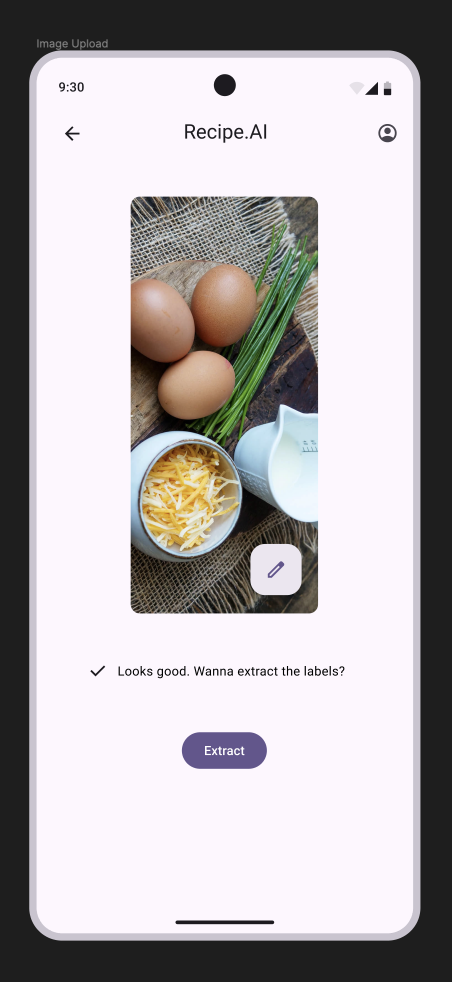
\includegraphics[width=0.25\textwidth]{pic3.png} \hspace{6mm}
        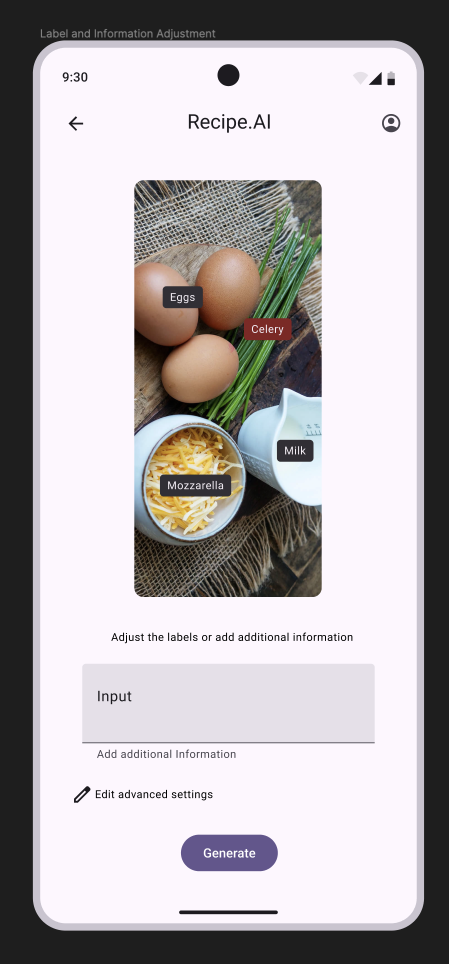
\includegraphics[width=0.25\textwidth]{pic4.png} \hspace{6mm}
        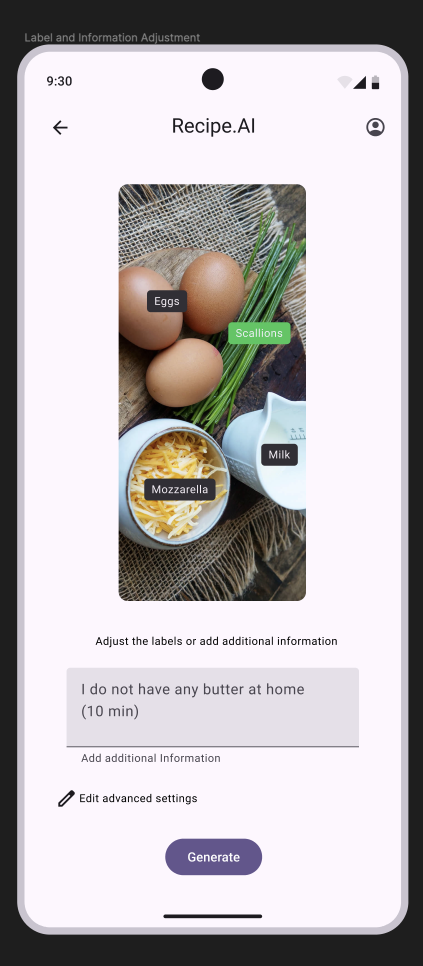
\includegraphics[width=0.237\textwidth]{pic5.png} 
    \end{center}
\end{frame}

%%%%%%%%%%%%%%%%%%%%%%%%%%%%%%%%%%%%%%%%%%%%%%%%%%%%%%%%%%%%%%%

\begin{frame}{Potential Applications (1)}
  \begin{flushleft}
    \textbf{Smart Cooking Guide}\\
    Personalized step‐by‐step instructions based on ingredients
  \end{flushleft}\vspace{4mm}
  \begin{flushright}
    \textbf{Fast Cooking}\\
    Instant recipe suggestions for meals under 15 minutes
  \end{flushright}
\end{frame}

\begin{frame}{Potential Applications (2)}
  \begin{flushleft}
    \textbf{Meal Planning \& Tracking}\\
    Auto‐generate weekly menus from photos
  \end{flushleft}\vspace{4mm}
  \begin{flushright}
    \textbf{Minimalist Recipes}\\
    Create tasty dishes using only 3--5 ingredients on hand
  \end{flushright}
\end{frame}

%%%%%%%%%%%%%%%%%%%%%%%%%%%%%%%%%%%%%%%%%%%%%%%%%%%%%%%%%%%%%%%

\begin{frame}{Value Proposition}
  \begin{center}
    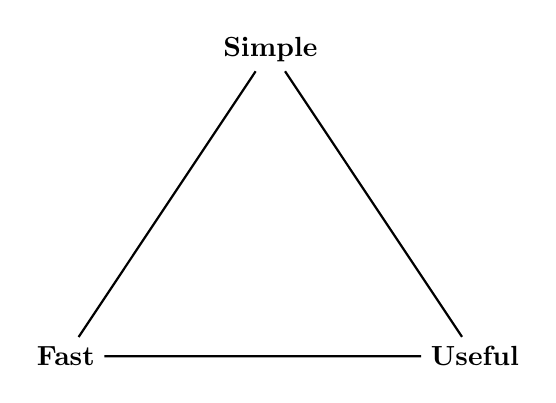
\begin{tikzpicture}[scale=2]
    
      % vertices
      \node (A) at (90:1.2cm)  {\textbf{Simple}};
      \node (B) at (210:1.5cm) {\textbf{Fast}};
      \node (C) at (-30:1.5cm) {\textbf{Useful}};
      % draw all three edges
      \draw[thick] (A) -- (B) -- (C) -- cycle;
      \draw[thick] (C) -- (A);
    \end{tikzpicture}
  \end{center}
\end{frame}







\section{Front End}

\begin{frame}{App Structure}
    \begin{center}
        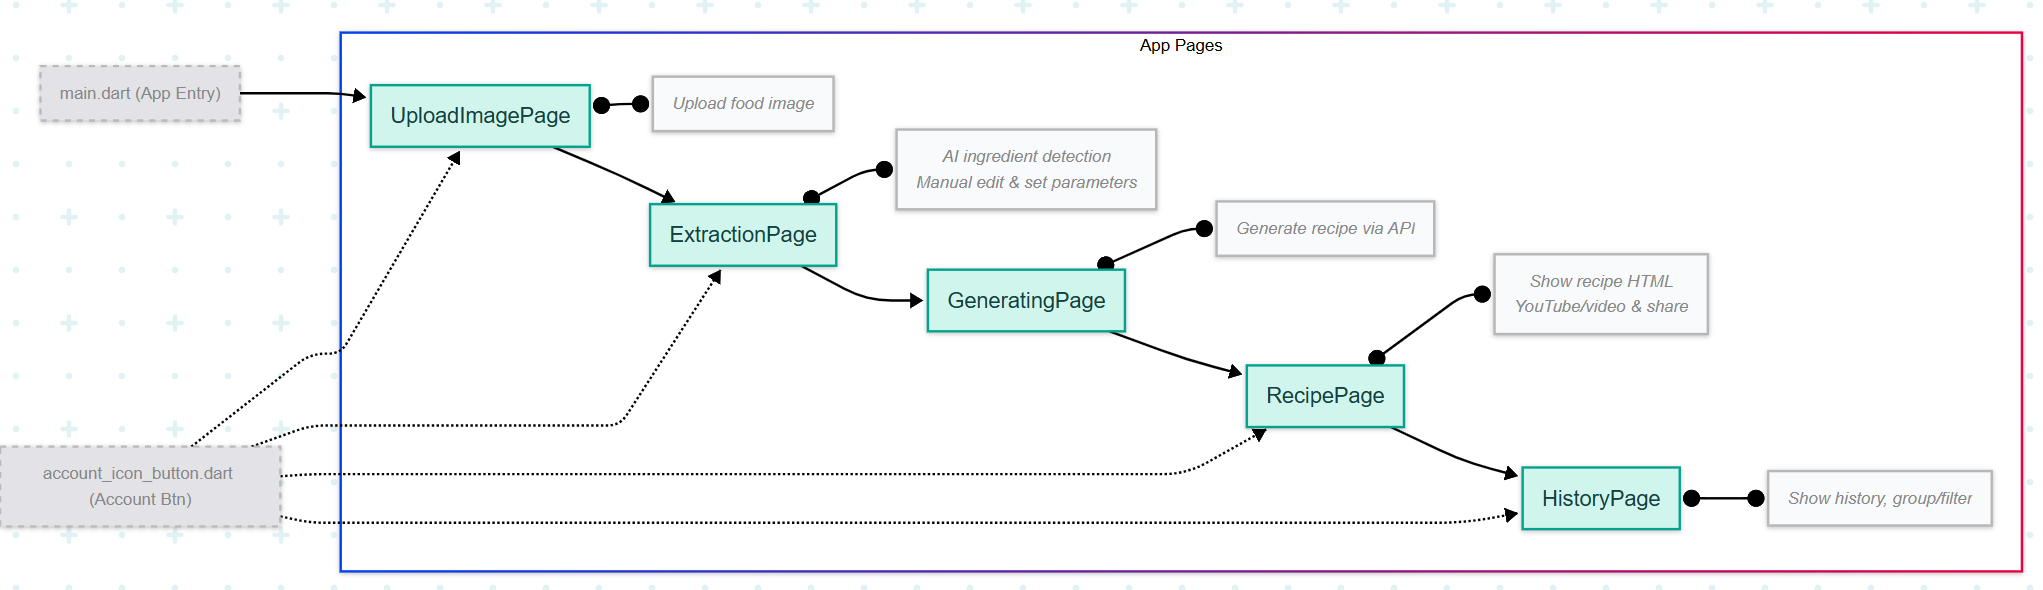
\includegraphics[width=1.0\textwidth, height=0.6\textheight]{frontend.png}

    \end{center}
\end{frame}

\begin{frame}{Initial Page}
    \begin{center}
        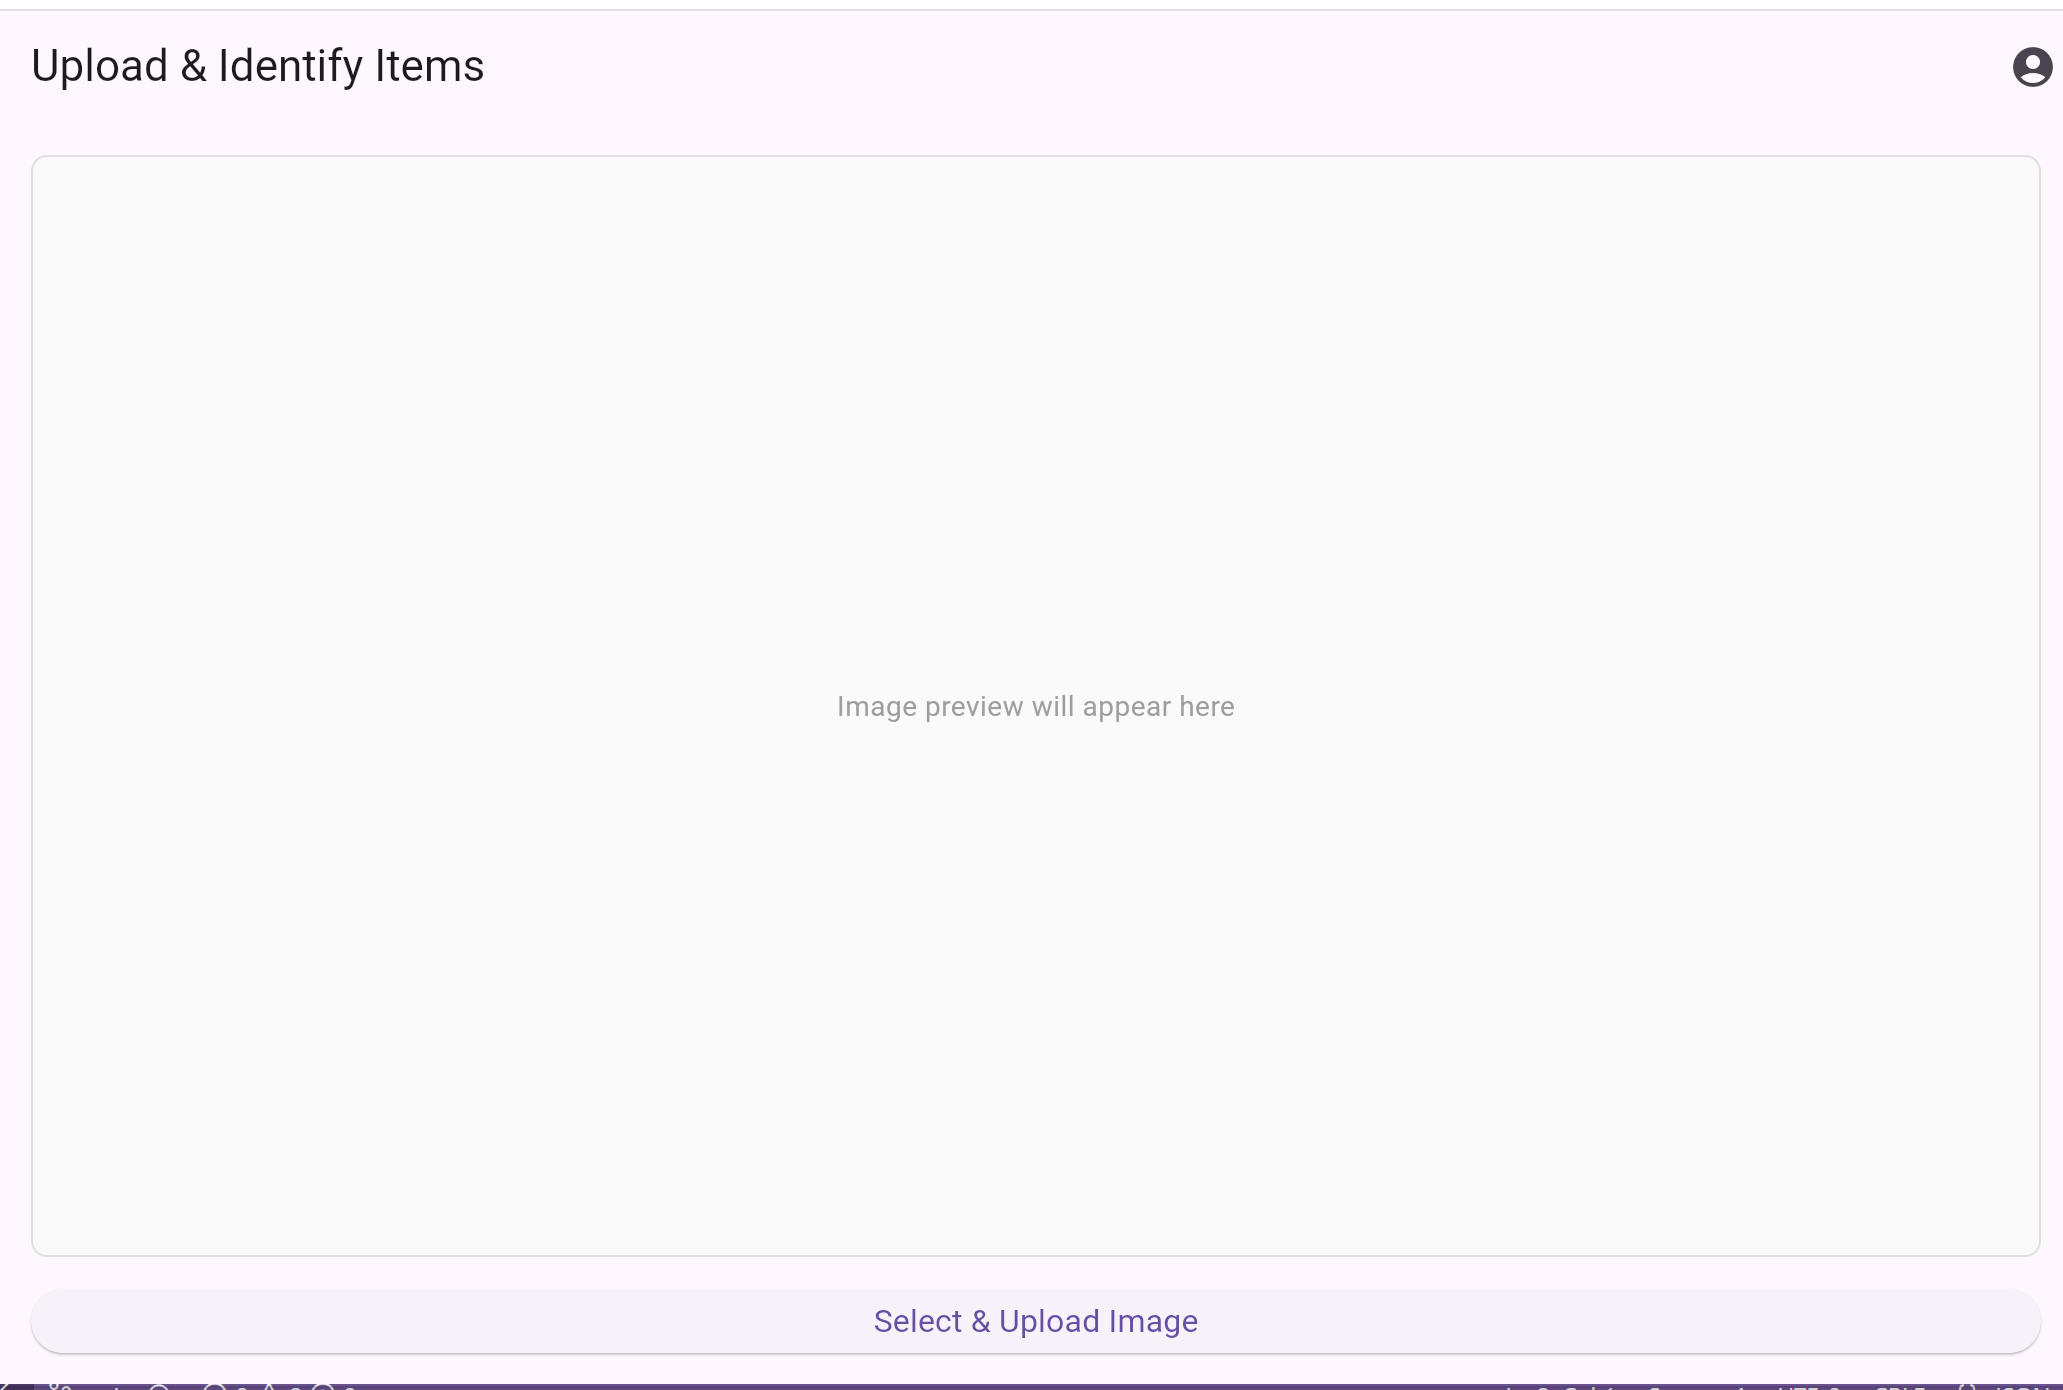
\includegraphics[width=0.95\textwidth,height=0.58\textheight,keepaspectratio]{initial_page.png}
    \end{center}
    \vspace{2mm}
    \begin{itemize}
        \item \small Unlogged-in user selects and uploads a food image to start the process.
    \end{itemize}
\end{frame}

\begin{frame}{Log-in Page}
    \begin{center}
        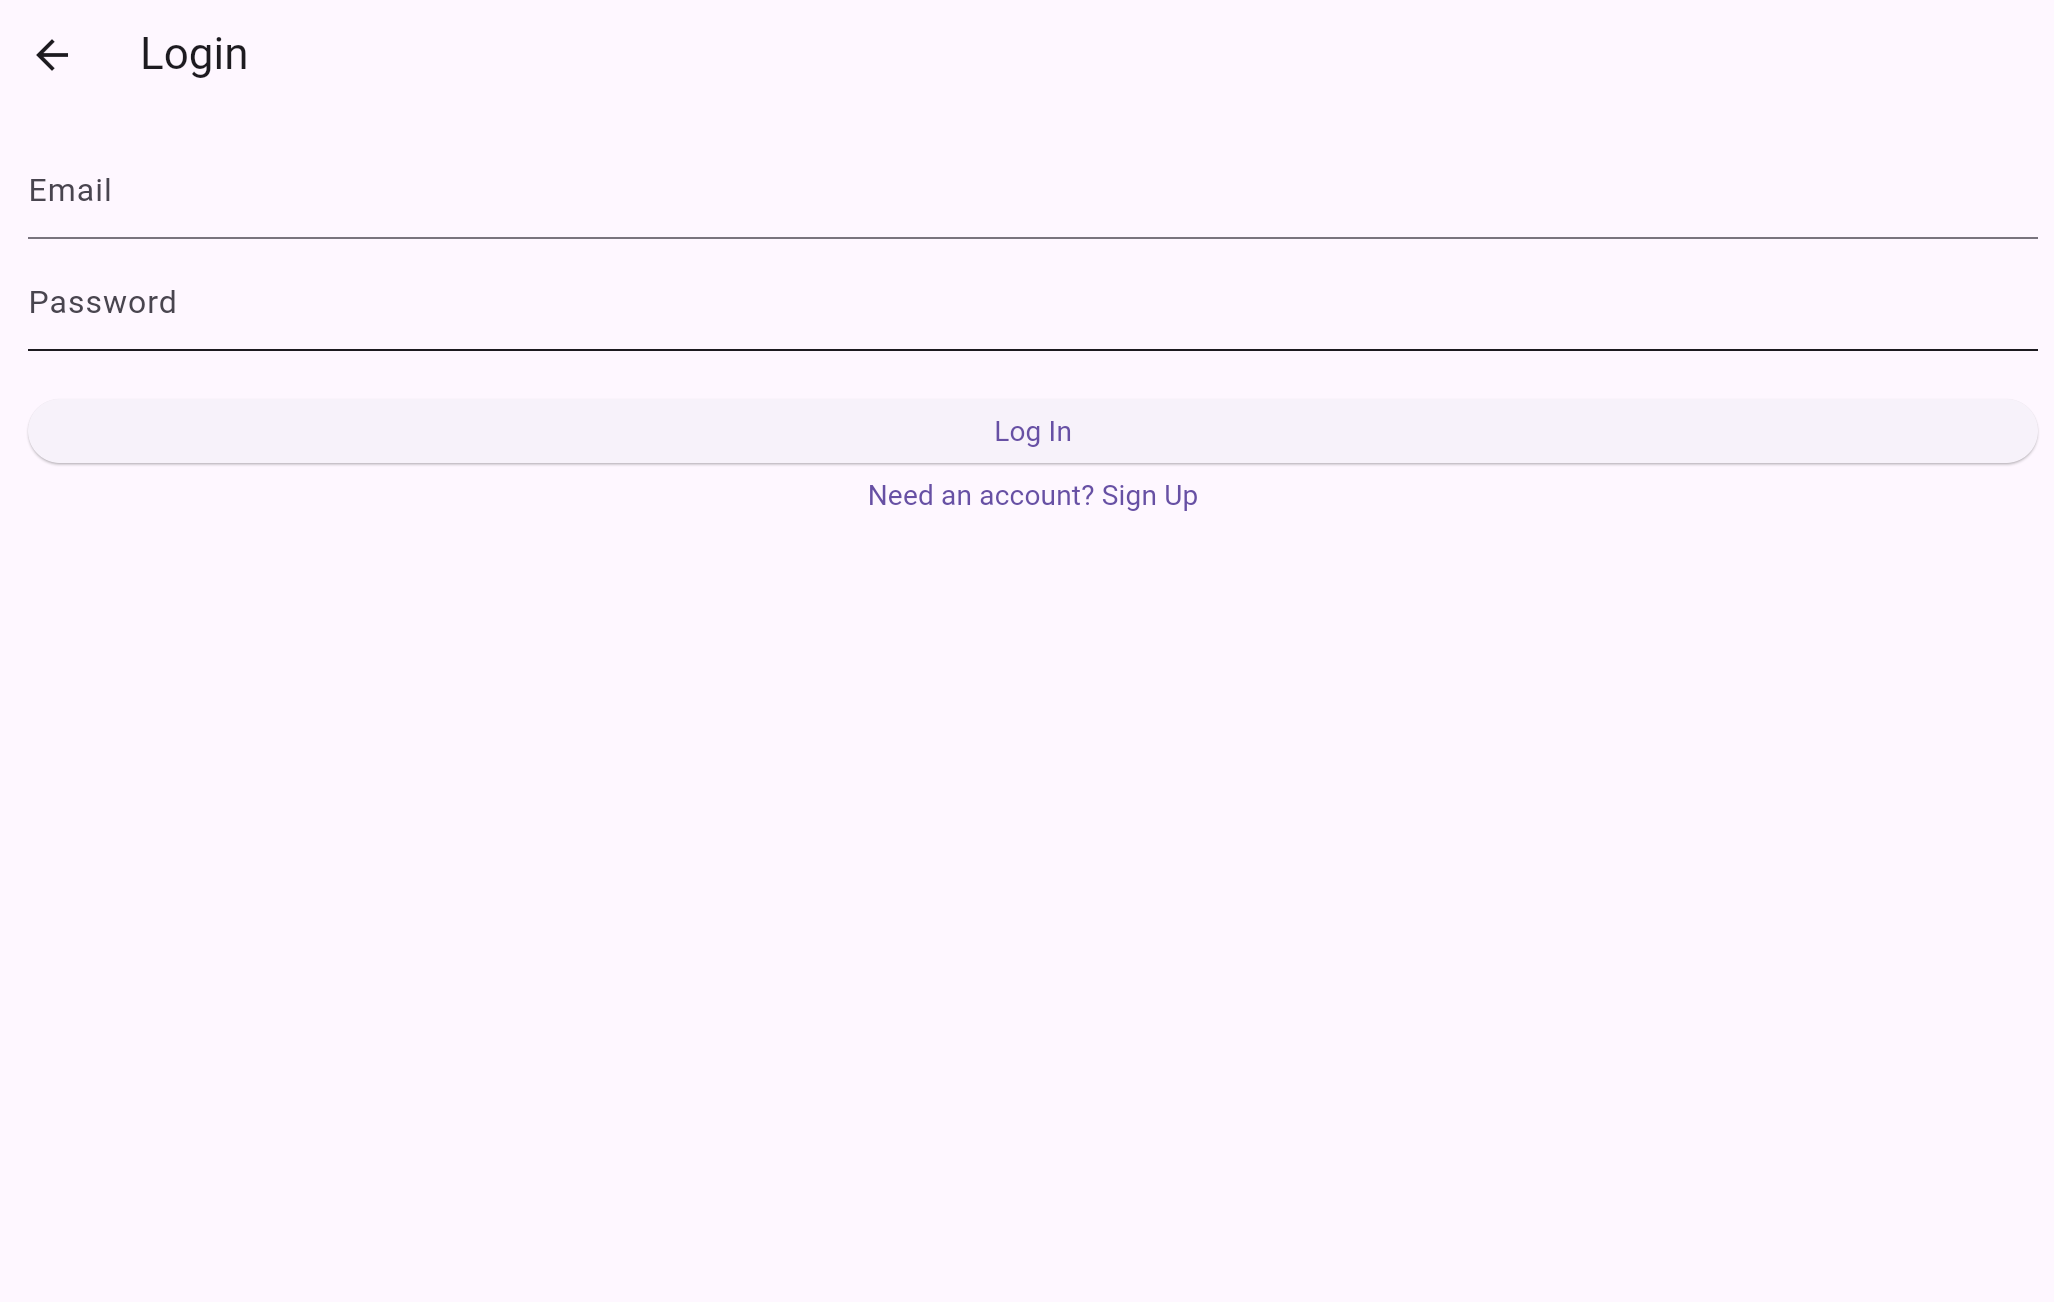
\includegraphics[width=0.95\textwidth,height=0.58\textheight,keepaspectratio]{login_page.png}
    \end{center}
    \vspace{2mm}
    \begin{itemize}
        \item \small Users can securely log in or sign up with their email and password to access personal features like history.
    \end{itemize}
\end{frame}

\begin{frame}{Upload Page}
    \begin{center}
        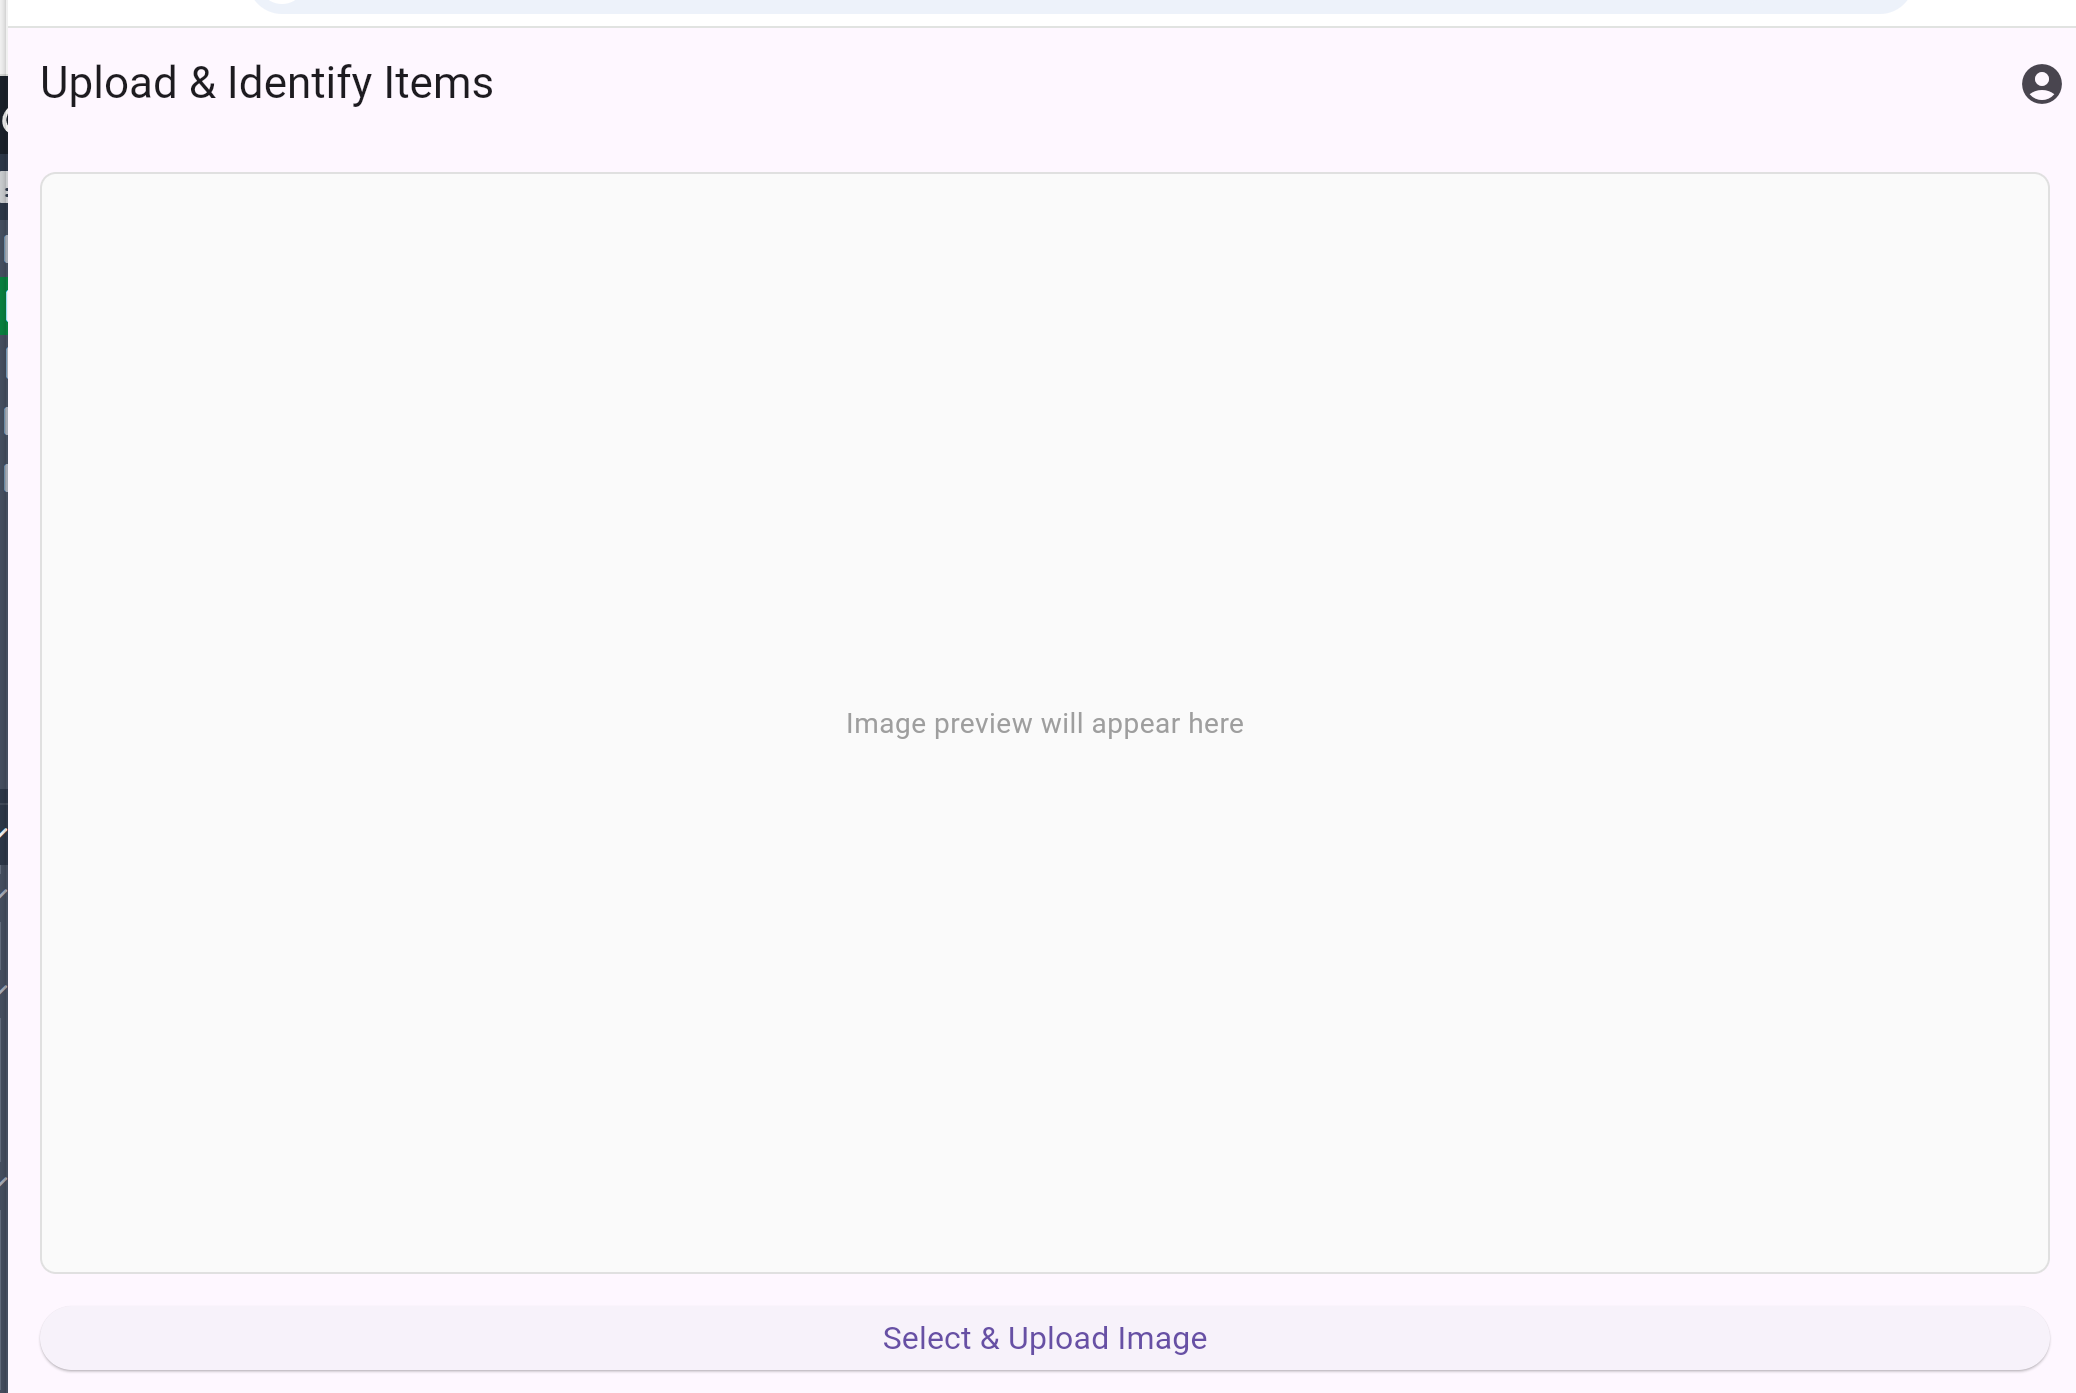
\includegraphics[width=0.95\textwidth,height=0.58\textheight,keepaspectratio]{upload_page.png}
    \end{center}
    \vspace{2mm}
    \begin{itemize}
        \item \small Logeed users select and upload a food image to start the recipe generation process.
    \end{itemize}
\end{frame}

\begin{frame}{Extraction Page}
    \begin{center}
        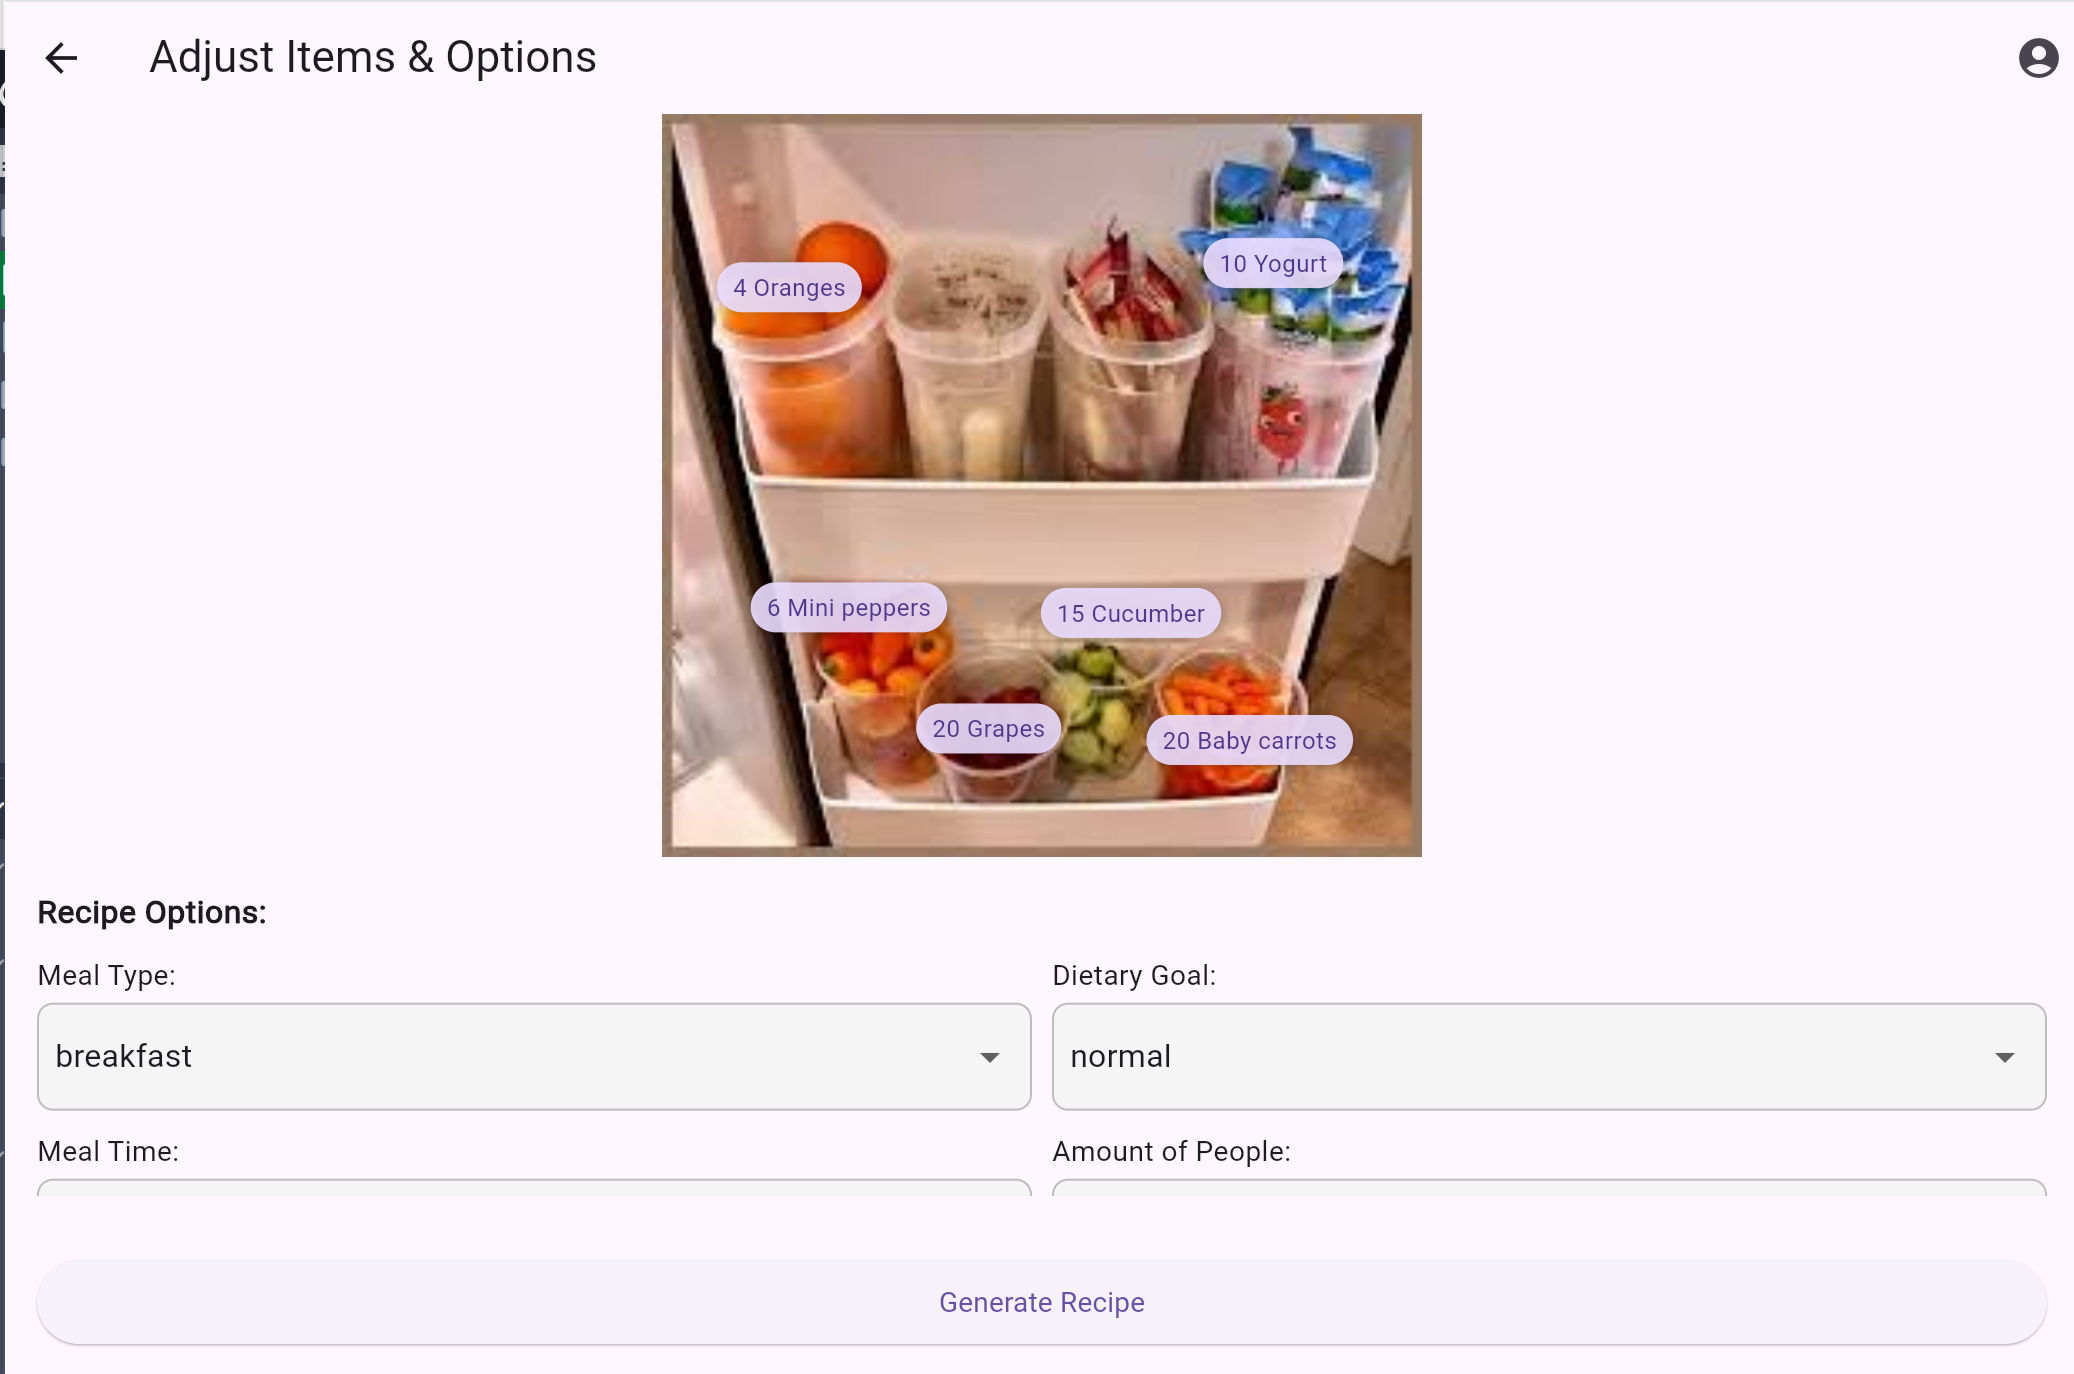
\includegraphics[width=0.95\textwidth,height=0.58\textheight,keepaspectratio]{extraction_page.png}
    \end{center}
    \vspace{2mm}
    \begin{itemize}
        \item \small Users review and adjust AI-detected ingredients, and set preferences for the recipe.
    \end{itemize}
\end{frame}

\begin{frame}{Generating Page}
    \begin{center}
        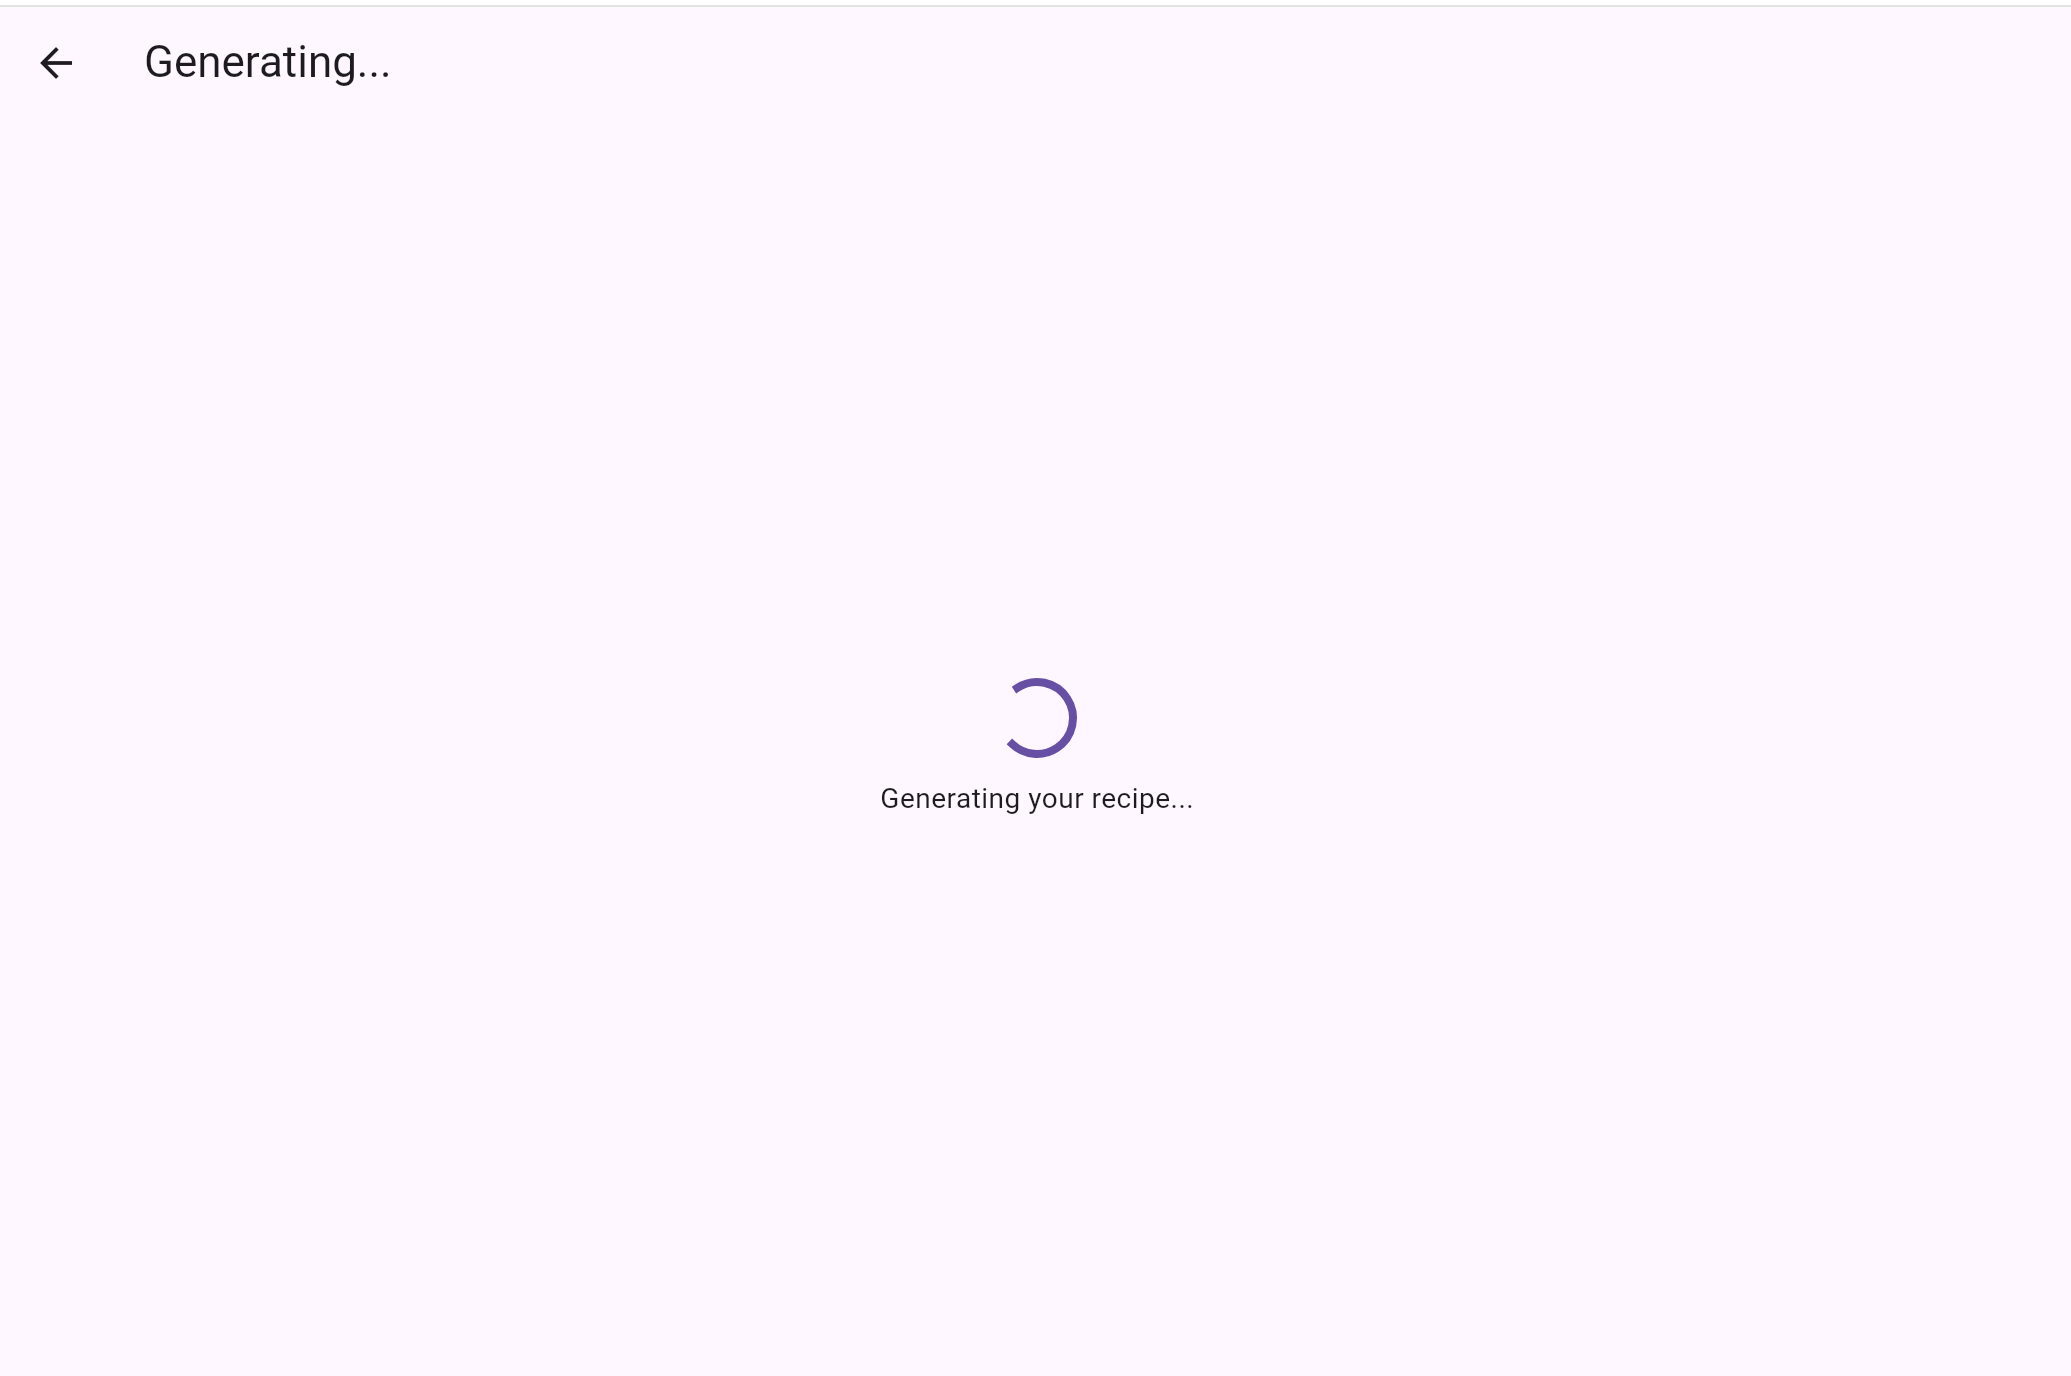
\includegraphics[width=0.95\textwidth,height=0.58\textheight,keepaspectratio]{generating_page.png}
    \end{center}
    \vspace{2mm}
    \begin{itemize}
        \item \small The app calls the edge function from backend to generate a recipe based on the selected ingredients and user preferences.
    \end{itemize}
\end{frame}

\begin{frame}{Recipe Page}
    \begin{center}
        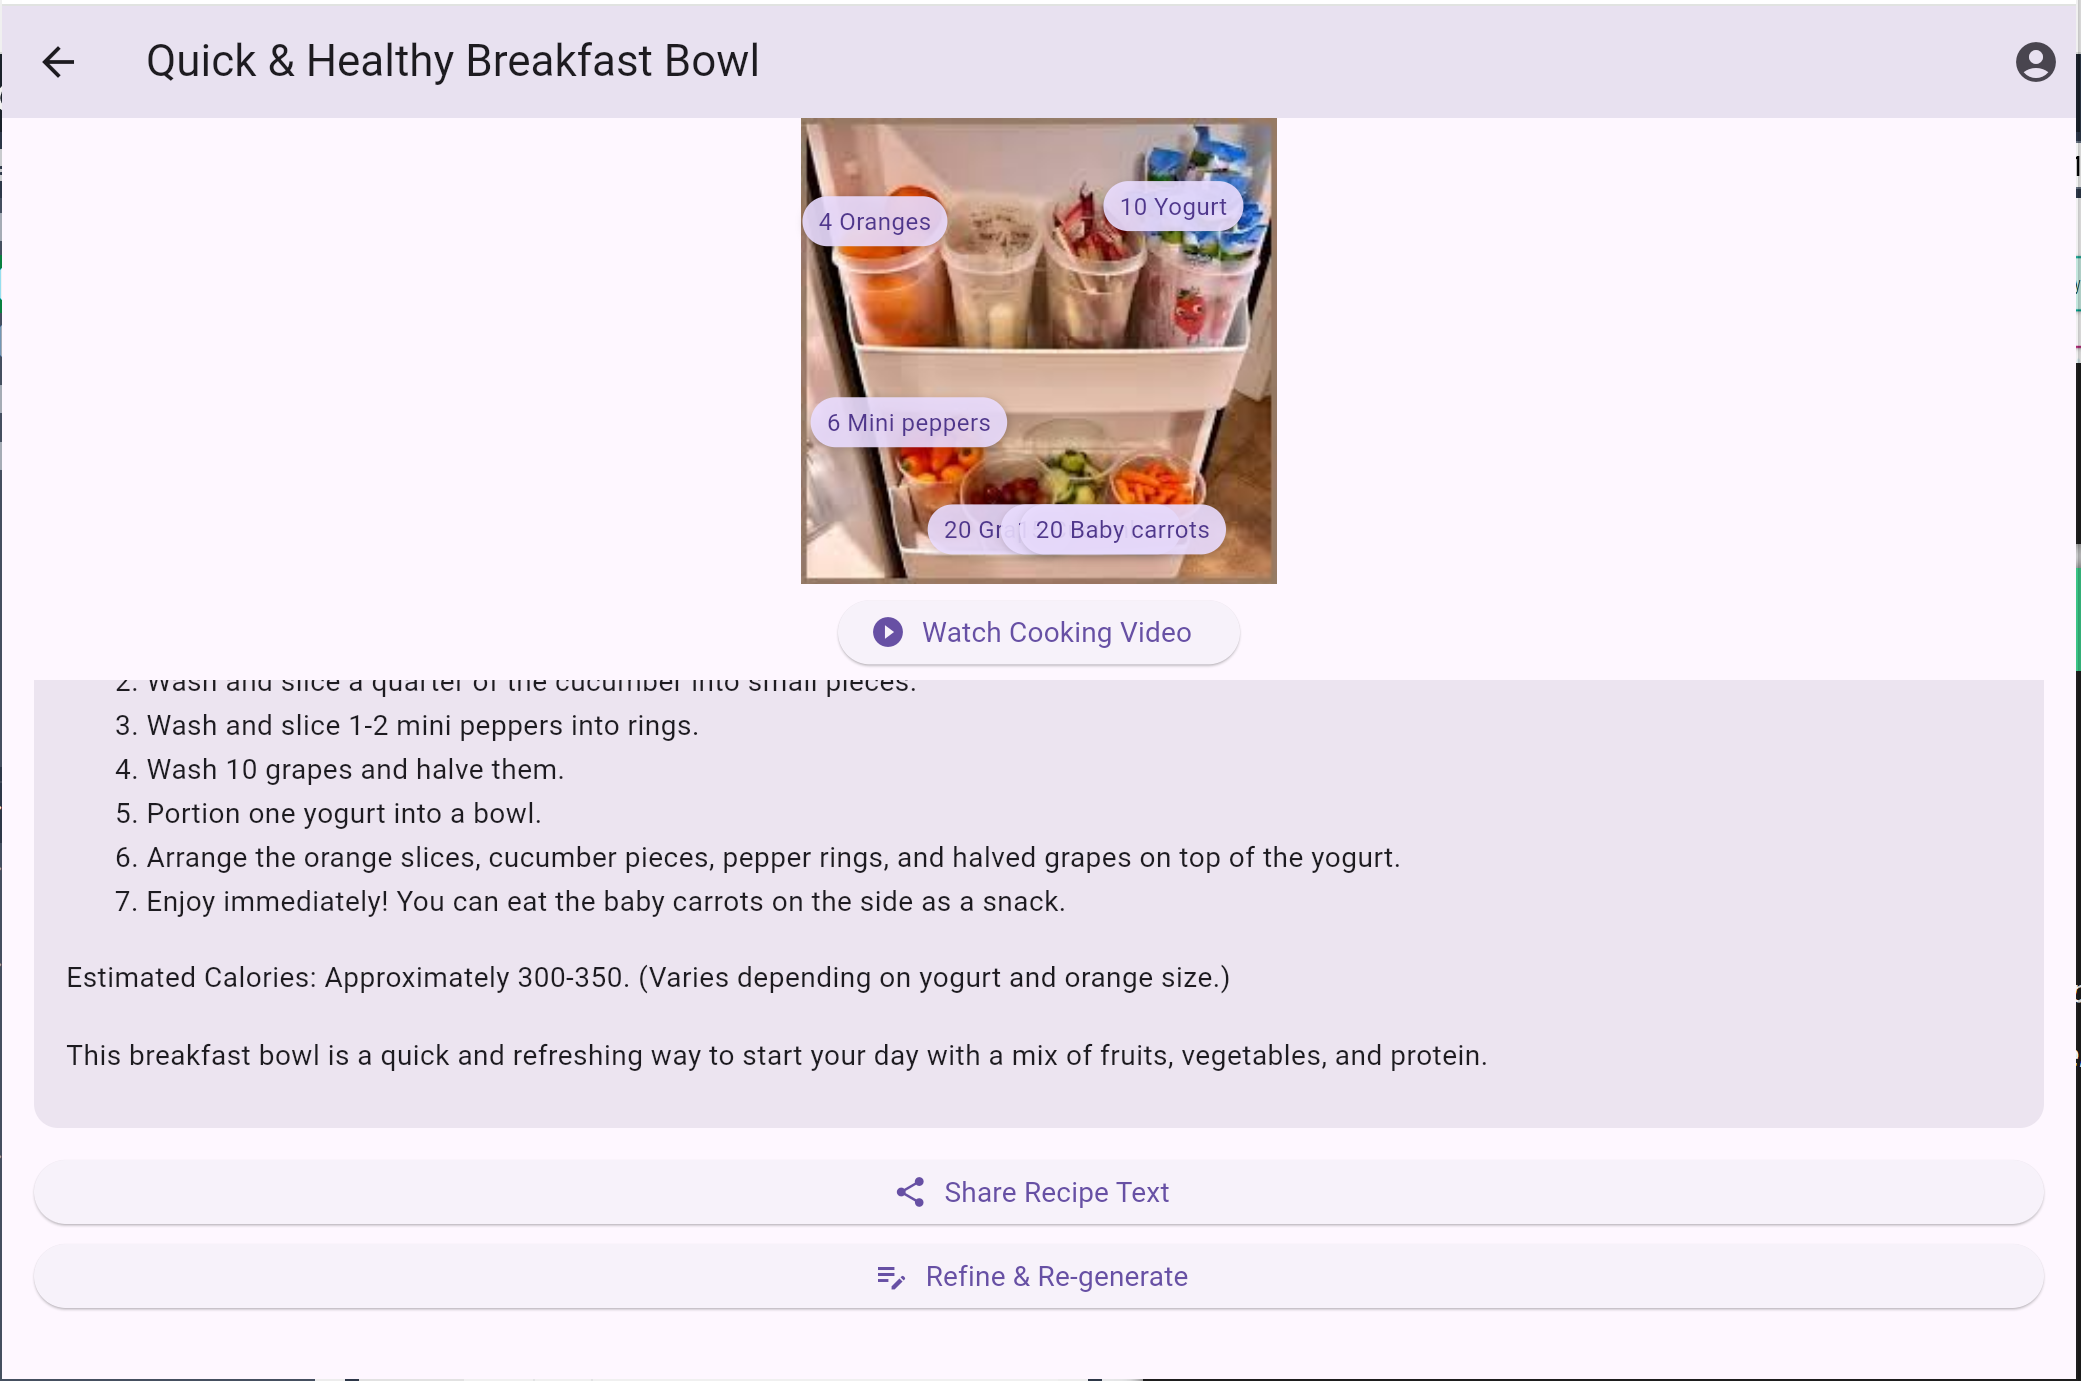
\includegraphics[width=0.95\textwidth,height=0.58\textheight,keepaspectratio]{recipe_page.png}
    \end{center}
    \vspace{2mm}
    \begin{itemize}
        \item \small Shows the generated recipe with steps, nutrition info, a video link, and sharing options.
    \end{itemize}
\end{frame}

\begin{frame}{History Page}
    \begin{center}
        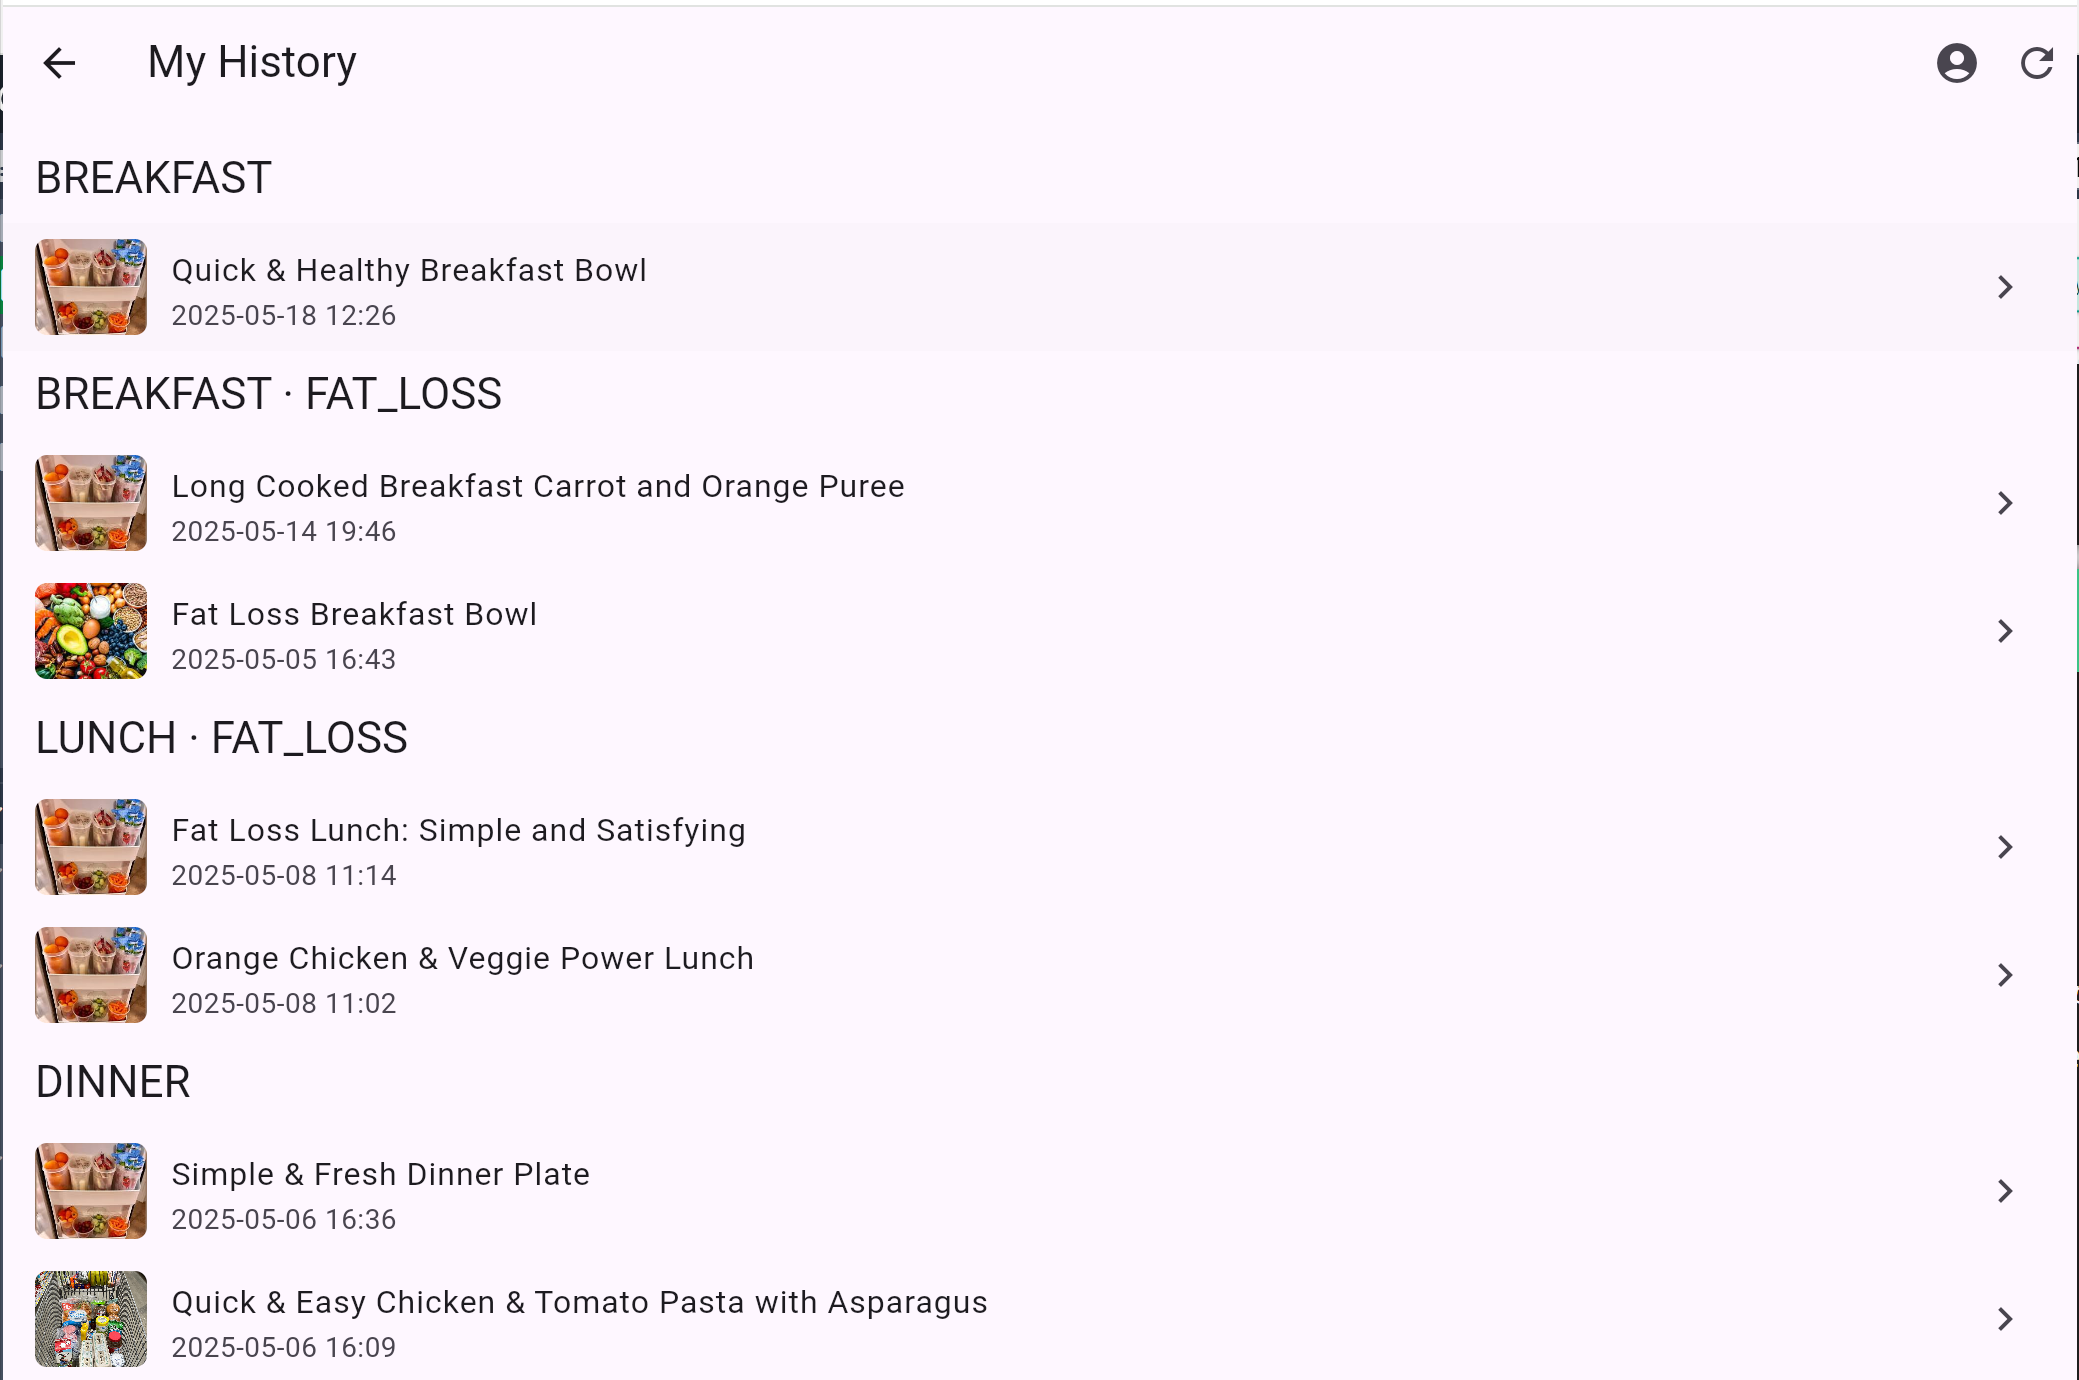
\includegraphics[width=0.95\textwidth,height=0.58\textheight,keepaspectratio]{history_page.png}
    \end{center}
    \vspace{2mm}
    \begin{itemize}
        \item \small Displays your recipe history, grouped by meal type and dietary tags for easy access.
    \end{itemize}
\end{frame}

\begin{frame}{History Table}
    \begin{center}
        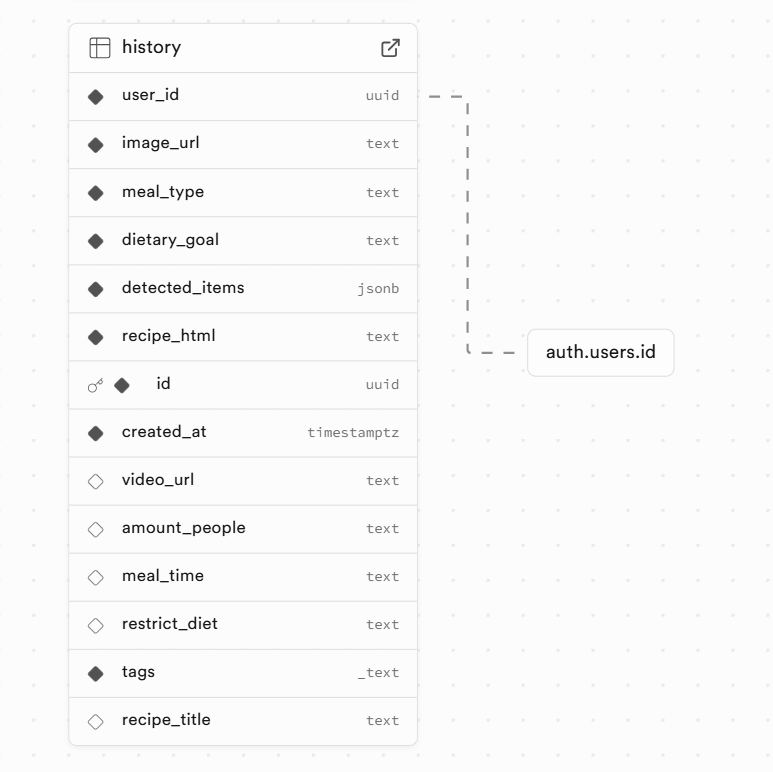
\includegraphics[width=0.95\textwidth,height=0.58\textheight,keepaspectratio]{table.png}
    \end{center}
    \vspace{2mm}
    \begin{itemize}
        \item \small All recipe generations are stored in a structured table, linked to user accounts, with key fields for filtering and display.
    \end{itemize}
\end{frame}


\section{Back End}

\begin{frame}{First Question: How do we develop the Backend?}
    % Replace your original enumerate with this table
    \begin{tabular}{|p{0.3\textwidth}|p{0.3\textwidth}|p{0.3\textwidth}|}
        \hline
        \textbf{Consideration} & \textbf{Custom Backend} & \textbf{Out-of-the-Box Solution} \\
        \hline
        \textbf{Customizability} & High & Moderate to High \\
        \hline
        \textbf{Time Investment} & Significant (Dev + Ops) & Low (Setup + Config) \\
        \hline
        \textbf{Opportunity Cost} & Higher (focus on infrastructure) & Lower (focus on core product) \\
        \hline
        \textbf{Pricing Model} & Variable (infra + dev) & Often Tiered (Free to Enterprise) \\
        \hline
        \textbf{Open-Source Nature} & Own Code & Varies (some are, some aren't) \\
        \hline
    \end{tabular}
\end{frame}

\begin{frame}{How Supabase addresses these questions}
    \begin{block}{\textbf{Benefits of using Supabase 
\includegraphics[width=0.05\textwidth]{pic2.jpeg}}}
        \begin{enumerate}
            \item Rich out-of-the-box functionality
            \item Low time-investment
            \item Focus on core product features instead of infrastructure (Automated hosting by Supabase)
            \item Generous free tier
            \item Open-source code
        \end{enumerate}
    \end{block}
\end{frame}

\begin{frame}{Second Question: How do we extract the labels and generate the recipe?}
    \begin{block}{\textbf{\textcolor{white}{Process Overview: From Image to Recipe}}}
        \centering
        \vspace{2mm}
        \begin{tikzpicture}[
            node distance=0.7cm, % Horizontal distance between nodes
            vertical node distance=0.7cm, % Vertical distance between rows
            block/.style={
                rectangle, draw, fill=blue!10, text width=2.8cm, align=center, minimum height=1.5cm, rounded corners
            },
            process/.style={
                rectangle,
                draw=black!50,
                fill=green!25!white,
                text width=2.4cm,
                align=center,
                minimum height=1.6cm,
                rounded corners,
                font=\small\color{black}
            },
            io/.style={
                rectangle,
                draw=black!50,
                fill=pink!40,
                text width=2.1cm,
                align=center,
                minimum height=1.6cm,
                rounded corners,
                font=\small\color{black}
            },
            arrow/.style={
                -Latex,
                thick,
                draw=black!70
            },
            arrowlabel/.style={
                font=\footnotesize\color{white},
                fill=white,
                opacity=0.8,
                text opacity=1
            }
        ]
            % First Row
            \node (input) [io] {Grocery\\Item Image};
            \node (extract) [process, right=of input] {LLM: Label\\Extraction};

            % Second Row
            % Position 'display' relative to 'input' for better vertical alignment
            \node (display) [process, below=of input.south west, anchor=north west, xshift=3.1cm] {Display Labels\\on App};
            \node (generate) [process, right=of display] {LLM: Recipe\\Generation};

            % Third Row
            % Place 'output' below 'generate' (or centered below the previous row's flow)
            \node (output) [io, below=of generate.south, anchor=north] {Generated\\Recipe};

            % Arrows
            \draw [arrow] (input) -- (extract);
            % Arrow from extract to display
            \draw [arrow] (extract.south) -- (display.north) node[midway, left, font=\footnotesize, color=white, xshift=-0.1cm] {Extracted Labels};
            \draw [arrow] (display) -- (generate);
            % Arrow from generate to output (vertical)
            \draw [arrow] (generate.south) -- (output.north) node[midway, left, font=\footnotesize, color=white, xshift=-0.1cm] {Recipe text};
        \end{tikzpicture}
    \end{block}
\end{frame}


\begin{frame}{How can we extract the labels consistently?}
    \begin{block}{\textbf{The magic happens through Prompt Engineering:}}
        \begin{itemize}
            \item \textbf{Precision in Detection:}
            \begin{quote}
                \vspace{0.2cm}
                "Only include items that are clearly identifiable as food. Ignore any non-food items or objects whose edibility is ambiguous."
            \end{quote}
            \item \textbf{Focus on the Item, Not Packaging:}
            \begin{quote}
                \vspace{0.2cm}
                "Don't include information about the packaging... We are interested in the item itself, not the container."
            \end{quote}
            \item \textbf{Structured and Reliable Output:}
            \begin{quote}
                \vspace{0.2cm}
                "Return results in valid JSON, no extra text. Ensure 'quantity' is an integer."
            \end{quote}
        \end{itemize}
    \end{block}
\end{frame}

\begin{frame}{The End}
    \textbf{Thank you for listening!}
\end{frame}

\end{document}